\documentclass{article}
\usepackage[OT1]{fontenc}
\usepackage[utf8]{inputenc}
\usepackage{amsthm,amssymb,amsmath}
\usepackage[a4paper, total={6.5in, 9in}]{geometry}
\usepackage[compact,explicit]{titlesec}
\usepackage[greek,english]{babel}
%\usepackage[iso-8859-7]{inputenc}
\usepackage[table]{xcolor}
%\usepackage{amsfonts}
%\usepackage{amsmath}
\usepackage{amssymb}
\usepackage{amsmath}
\usepackage{pgfplots}
\usepackage{tikz}
\usepackage{tikzscale}
\usepackage{array}
\usepackage{booktabs}
\usepackage{enumerate}
%\usepackage{color}
%AASFASFASF
\usepackage{empheq}
\usepackage{enumerate}
\usepackage{enumitem}
%\usepackage{gensymb}
\usepackage{graphicx}
\usepackage[space]{grffile}
\usepackage{ifthen}
%\usepackage{kerkis}
\usepackage{marginnote}
\usepackage{mathtools}
\usepackage{mdframed}
\usepackage{multirow}
%\usepackage{textgreek}
\usepackage{float}
\usepackage{slashbox}
\usepackage{listings}

\usepackage{caption}
\usepackage{afterpage}
\usepackage{forloop}
\usepackage{systeme}
\usepackage{cancel}
\usepackage{subcaption}
\usepackage{hyperref}
\usepackage{tikzsymbols}
\usetikzlibrary{calc}
\usepackage{changes}
\usepackage{cancel}
\setdeletedmarkup{\cancel{#1}}
%\usepackage{bbold}
%\newtheorem*{theorem}{Theorem}




\newcommand{\NN}{\mathbb{N}}
\newcommand{\ZZ}{\mathbb{Z}}
\newcommand{\RR}{\mathbb{R}}
\newcommand{\RRp}{\mathbb{R}^{+}}
\newcommand{\RRpp}{\mathbb{R}^{++}}
\newcommand{\QQ}{\mathbb{Q}}
\newcommand{\CC}{\mathbb{C}}
\newcolumntype{P}[1]{>{\centering\arraybackslash}p{#1}}

\newcommand{\tl}[1]{\textlatin{#1}}
\renewcommand\thesubfigure{(\roman{subfigure})}\usepackage{pgf, tikz}

\setlength{\arrayrulewidth}{1mm}
\setlength{\tabcolsep}{18pt}
\renewcommand{\arraystretch}{1.5}


\newcommand\blankpage{%
	\null
	\thispagestyle{empty}%
	\addtocounter{page}{-1}%
	\newpage}

\newcommand{\thewr}[1]{\mathrm{\ifthenelse{\equal{#1}{}}{}{#1,}\theta\epsilon\omega\rho}}
\newcommand{\peir}[1]{\mathrm{\ifthenelse{\equal{#1}{}}{}{#1,}\pi\epsilon\iota\rho}}
%\newcommand{\Upd}{\operatorname{U}^{\mathrm{M}}_{#1}}

\newlength\dlf
\newcommand\alignedbox[2]{
	% #1 = before alignment
	% #2 = after alignment
	&
	\begingroup
	\settowidth\dlf{$\displaystyle #1$}
	\addtolength\dlf{\fboxsep+\fboxrule}
	\hspace{-\dlf}
	\boxed{#1 #2}
	\endgroup
}

\setlist{  
	listparindent=\parindent%,
	%parsep=0pt
}

\hypersetup{
	colorlinks,
	linkcolor={red!50!black},
	citecolor={blue!50!black},
	urlcolor={blue!80!black}
}



%\let\thetitle\@title
%\let\theauthor\@author
%\let\thedate\@date

\DeclarePairedDelimiter\ceil{\lceil}{\rceil}

\DeclareMathOperator*{\argmax}{argmax} % thin space, limits underneath in display
\makeatother

\allowdisplaybreaks

%Η απόλυτη τιμή
\DeclarePairedDelimiter\abs{\lvert}{\rvert}


\renewcommand{\theenumi}{\roman{enumi}}
\begin{document}
	\greektext
	\captionsetup[figure]{labelfont={default},labelformat={default},labelsep=period,name={Σχήμα:}}
	\captionsetup[table]{labelfont={default},labelformat={default},labelsep=period,name={Πίνακας:}}
	\title{\tl{Assignment 3: Detection}}						% Title
	\author{Μαυρογιώργης Δημήτρης, AM:2016030016\\Κολομβάκη Αφροδίτη, AM:2016030158\\Δελατόλας Θάνος, AM:2016030074}								% Author
	\date{\today}											% Date
	
	\makeatletter
	\let\thetitle\@title
	\let\theauthor\@author
	\let\thedate\@date
	\makeatother
	
	
	
	\begin{titlepage}
		\centering
		\vspace*{0.5 cm}
		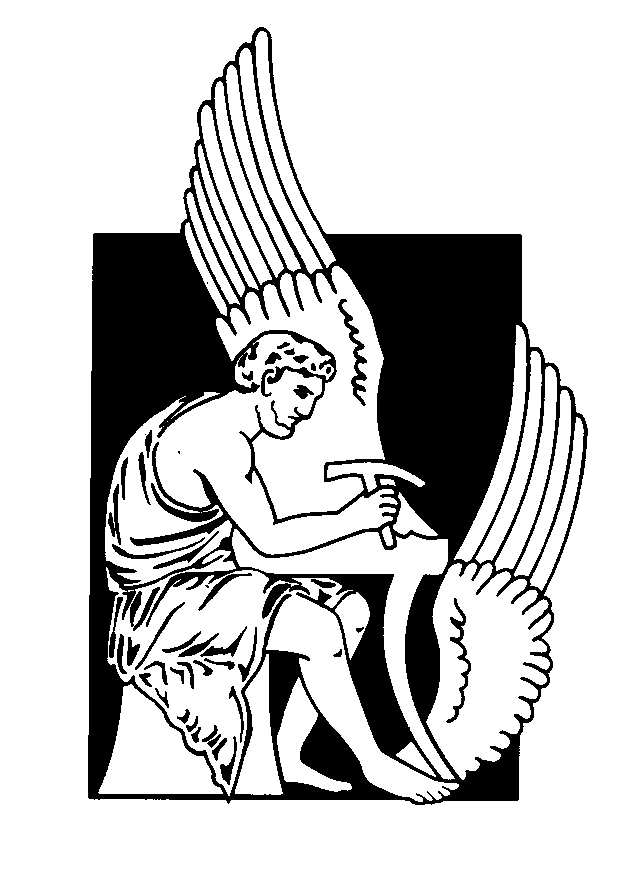
\includegraphics[scale = 0.4]{../../Assignment 1/report/polytexneio-logo.png}\\[1.0 cm]	% University Logo
		\textsc{\LARGE Μηχανικη Όραση }\\[2.0 cm]	
		\rule{\linewidth}{0.2 mm} \\[0.4 cm]
		{ \huge \bfseries \thetitle}\\
		\rule{\linewidth}{0.2 mm} \\[1.5 cm]
		
		\begin{minipage}{0.6\textwidth}
			
			\begin{flushright} \large
				\theauthor\\
				
			\end{flushright}
			
			\begin{flushright} \large
				\tl{\thedate}\\
				
			\end{flushright}
			
		\end{minipage}\\[2 cm]
		
	\end{titlepage}	
	\newpage
	\section*{1. \tl{Introduction}}
	Σκοπός της τρίτης εργαστηριακής άσκησης είναι να δημιουργήσουμε έναν \tl{object detector}, ο οποίος βασίζεται στην εξαγωγή χαρακτηριστικών με βάση 
	το \tl{Histograms of Gradient Orientations} και χρησιμοποιεί τη μέθοδο των \tl{sliding windows} για να κάνει \tl{classification}. Πιο συγκεκριμένα, 
	στόχος μας είναι να εξάγουμε κάποια \tl{positive} και κάποια \tl{negative} δείγματα από ένα \tl{set} εικόνων, να τις μετατρέψουμε σε ένα σύνολο 
	χαρακτηριστικών και να τα χρησιμοποιήσουμε για να κάνουμε \tl{train} το μοντέλο μας. Η εξαγωγή χαρακτηριστικών από τα δείγματα γίνεται με τη 
	αναπαράσταση \tl{HOG}, με την οποία βγάζουμε ένα \tl{feature vector}, το οποίο στη συνέχεια θα χρησιμοποιηθεί, για να γίνει το \tl{classification}.\\\\
	\section*{2. \tl{Implementation}}
	\begin{enumerate}[label=\arabic*.]
		\item \textbf{\tl{Image Gradient}} \\
		Αρχικά, επίλέξαμε ένα φίλτρο \tl{Sobel} \tl{3x3}, για να υπολογίσουμε τη συνέλιξη της εικόνας με το φίλτρο, επειδή το συγκεκριμένο φίλτρο 
		χρησιμοποιείται για τον υπολογισμό μιας προσεγγιστικής τιμής των παραγώγων. Πιο συγκεκριμένα, χρησιμοποιήσαμε το φίλτρο για να βρούμε τις 
		οριζόντιες και κατακόρυφες αλλαγές που υπάρχουν στην εικόνα. Τα φίλτρα που χρησιμοποιήσαμε για να βρούμε τις κατακόρυφες και οριζόντιες
		διαφορές είναι τα παρακάτω:
		\[
		G_y=\begin{bmatrix}
			-1 & -2 & -1\\
			0 & 0 & 0\\
			1 & 2 & 1
		\end{bmatrix} , \ \ \ G_x=\begin{bmatrix}
			-1 & 0 & 1\\
			-2 & 0 & 2\\
			-1 & 0 & 1
		\end{bmatrix}
		\]
		\\
		\noindent
		Το φίλτρο $G_x$ το δημιουργήσαμε στη \tl{matlab} με τη συνάρτηση \tl{fspacial} και το αποτέλεσμά της το πολλαπλασιάσαμε με -1 έτσι, ώστε να 
		προκύψουν οι αρνητικές τιμές από τα αριστερά και οι θετικές από δεξιά. Επιπλέον, το φίλτρο $G_y$ το υπολογίσαμε παίρνοντας τον ανάστροφο 
		πίνακα του $G_x$.
		\\
		\noindent
		Στη συγκεκριμένη συνάρτηση που υλοποιήσαμε, υπολογίζουμε τη συνέλιξη των παραπάνω φίλτρων με την εικόνα, ενώ υπολογίζουμε το magnitude και
		το orientation με βάση τους παρακάτω τύπους
		\begin{align*}
			||\nabla f|| &= \sqrt{D_{x}^2 + D_{y}^2}	\\ 
			\theta &= \tan^{-1}\left( \frac{D_{y}}{D_{x}}\right) 
		\end{align*}
		
		\item \textbf{\tl{Histograms of Gradient Orientations}} \\
		Στη συγκεκριμένη συνάρτηση υπολογίσουμε το \tl{gradient} της εικόνας και στη συνέχεια θέλουμε να βρούμε τα \tl{pixel} της εικόνας που έχουν 
		\tl{magnitude} πάνω από το 10\% του μέγιστου και το \tl{orientation} που ανήκει σε κάποιο από τα 9 \tl{bins} που έχουμε χωρίσει το διάστημα 
		$\left[ -\frac{\pi}{2}, \frac{\pi}{2} \right]$.\\
		
		\noindent
		Για την υλοποίηση, δημιουργείται ένας \tl{boolean array} για κάθε ένα από τα 9 \tl{bins.} Αν το στοιχείο \tl{(i,j)} είναι \tl{true}
		τότε το \tl{pixel (i,j)} έχει μια επιθυμητή τιμή \tl{magnitude} και το \tl{orientation} του είναι μέσα στο δίαστημα που ορίζεται από το 
		\tl{bin}. Τέλος, αθροίζουμε και τα 9 \tl{bins} του κάθε \tl{pixel} και κανονικοποιούμε στο διάστημα $\left[0,1\right]$, για να μην επηρρεαζόμαστε 
		από διάφορες αλλαγές στη φωτεινότητα της εικόνας.
		\\
		\item \textbf{\tl{Detection}} \\
		Αρχικά, υπολογίζεται το \tl{cross-correlation} μεταξύ του \tl{feature map} και του \tl{template}. Στη συνέχεια, σκοπός είναι να 
		βρούμε τα \tl{detection} που έχουν το μεγαλύτερο \tl{cross-correlation} και κατ' επέκταση το μικρότερο \tl{sum of square differences}. Για την υλοποίηση
		αυτού ταξινομήθηκαν τα \tl{cross-correlation} με φθίνουσα σειρά και αφαιρέθηκαν τα \tl{detection} που εχουν \tl{overlap} πάνω απο το 70\% του \tl{template width.}\\
		
		\noindent
		Ως \tl{detection} ορίζεται το σημείο \tl{(i,j)} του πίνακα \tl{cross-correlation} το οποίο είναι και κέντρο ενός \tl{block}. Για να μην υπάρχει \tl{overlap} πάνω από 
		το όριο που αναφέρθηκε παραπάνω, υπολογίζεται η Ευκλείδεια απόσταση μεταξύ του νέου σήμειου και κάθε σήμείου που υπάρχει ήδη στη λίστα με τα \tl{top detection}. Αν η απόσταση
		δεν ξεπερνά το παραπάνω όριο, τότε μπαίνει στη λίστα με τα \tl{top detection} και αυξάνουμε το συνολικό \tl{detection counter}. Tέλος, αυτό που κάνουμε σε περίπτωση που 
		δεν βρούμε τον επιθυμητό αριθμό από \tl{detections}, είναι να επιστρέψουμε μόνο τις τιμές από 1 εως \tl{detection counter}.
		
		\item \textbf{\tl{Detection Script}} \\
		Στο συγκεκριμένο \tl{script}, το οποίο είναι το \tl{main program} της εργασίας, έχουμε θέσει δυο μεταβλητές με τις οποίες καθορίζουμε το \tl{width} και \tl{height} του \tl{template} (γραμμές 26 και 27 αντίστοιχα). Από τις διαστάσεις του \tl{template} καθορίζονται και οι διαστάσεις του \tl{patch}. Στη συνέχεια υπολογίζουμε το αριστερό και δεξιό όριο του template, αλλά και των παραθύρων, τα κέντρα των οποίων υπολογίζουμε με τη συνάρητηση \tl{detect} που υλοποιήσαμε.\\\\
		
		\noindent
		Κατόπιν, η λογική του προγράμματος είναι η εξής: 
		\begin{enumerate}[label=\arabic*.]
			\item Διαβάζουμε μία εικόνα και επιλέγουμε έναν αριθμό από \tl{click} που θα δώσει ο χρήστης για τα \tl{positive templates}, τα οποία είναι τα αντικείμενα που θέλουμε 
			να αναγνωρίσουμε.
			\item Υπολογίζουμε το \tl{HOG} της \tl{train} εικόνας και κατόπιν υπολογίζουμε το μέσο όρο των \tl{positive teamplates}. 
			\item Επαναλαμβάνουμε τα παραπάνω 2 βήματα για να καθορίσουμε τα \tl{negative templates}, τα οποία είναι αντικείμενα στην εικόνα τα οποία δεν έχουν σχέση με αυτά που 
			θελόυμε να αναγνωρίσουμε. Παραδείγματος χάρη μπορεί να είναι ένα λευκό \tl{background}.
			\item Ως \tl{template} ορίζουμε τη διαφορά μεταξύ \tl{avarage positive template} και \tl{negative template}.
			\item Τέλος, διαβάζουμε και μία άλλη \tl{test image} και χρησιμοποιούμε το \tl{template}, για να αναγνωρίσουμε σε αυτή την εικόνα τα αντικείμενα που επιλέξαμε στο πρώτο 
			βήμα του αλγορίθμου.
		\end{enumerate}
		\ \\
		\noindent
		Αφού μας επιστραφούν τα κέντρα από τη \tl{detect} ζωγραφίζουμε τα \tl{rectangles} στην ίδια εικόνα που διαβάσαμε ως \tl{test image}.
	\end{enumerate}
	\section*{3. \tl{Results}}
	\begin{figure}[H]
		\centering
		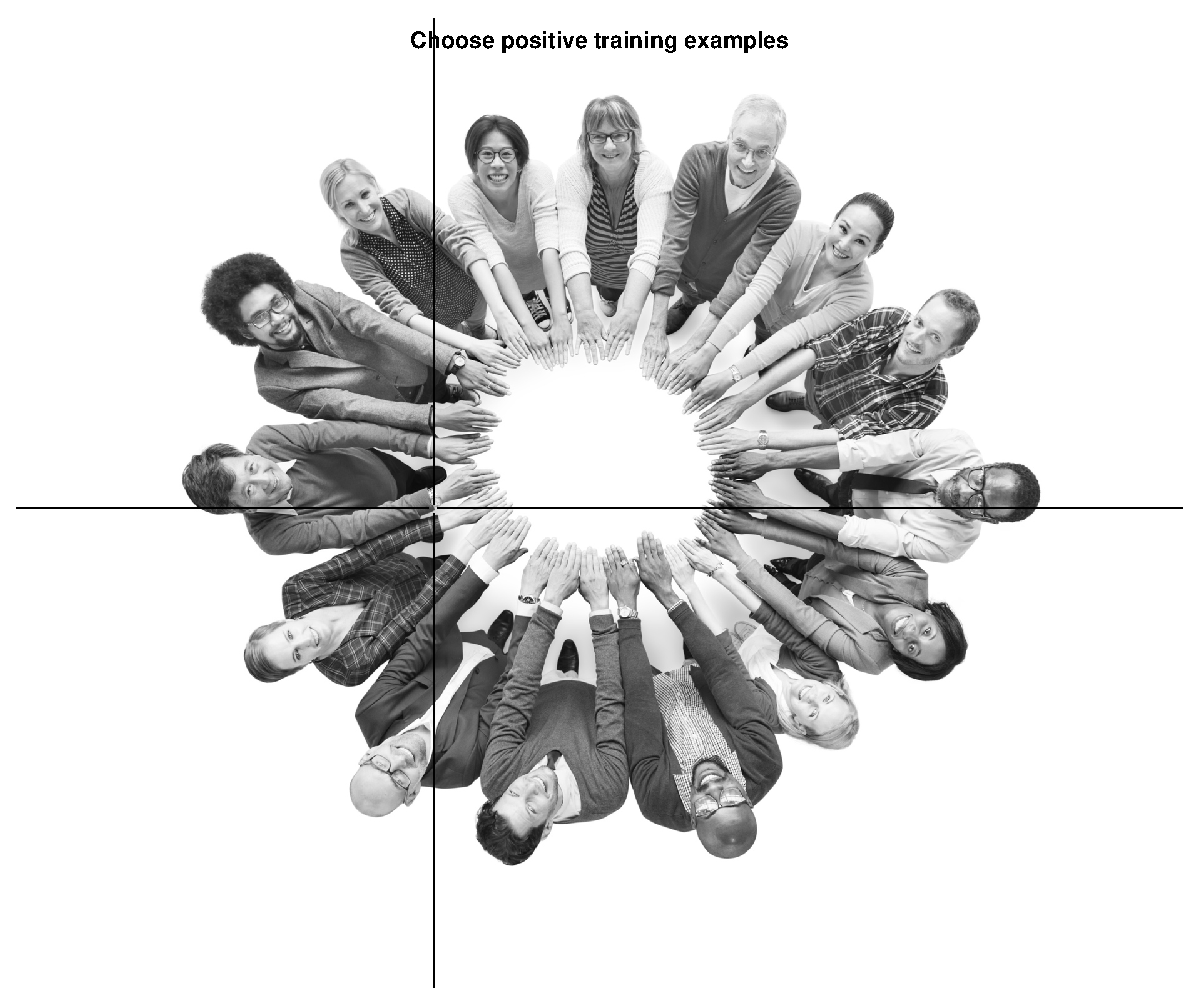
\includegraphics[scale=0.4]{res/input_image.eps}
		\caption{\tl{Input image}}
	\end{figure}%
	\begin{figure}[H]		
		\begin{subfigure}[b]{0.5\textwidth}
			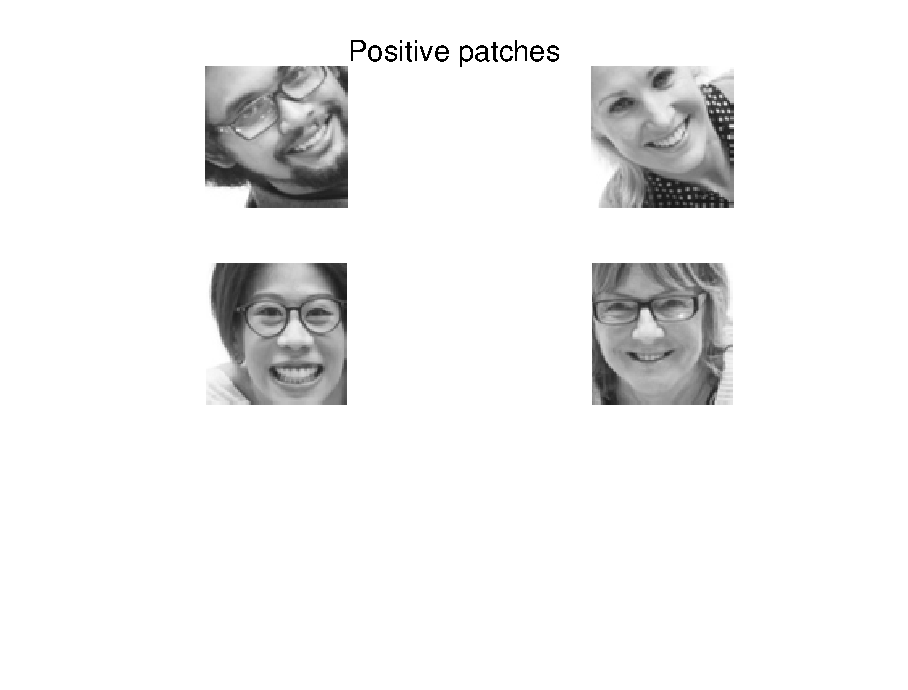
\includegraphics[width=\textwidth]{res/pos_patches.eps}
			\caption{Πρόσωπα προς εντοπισμό.}
			\label{fig:i}		
		\end{subfigure}%		
		\begin{subfigure}[b]{0.5\textwidth}
			
\includegraphics[width=\textwidth]{res/neg_patches.eps}
			\caption{Μη επιθυμητά αντικείμενα.}
		\end{subfigure}%
		
		\begin{subfigure}[b]{0.5\textwidth}
			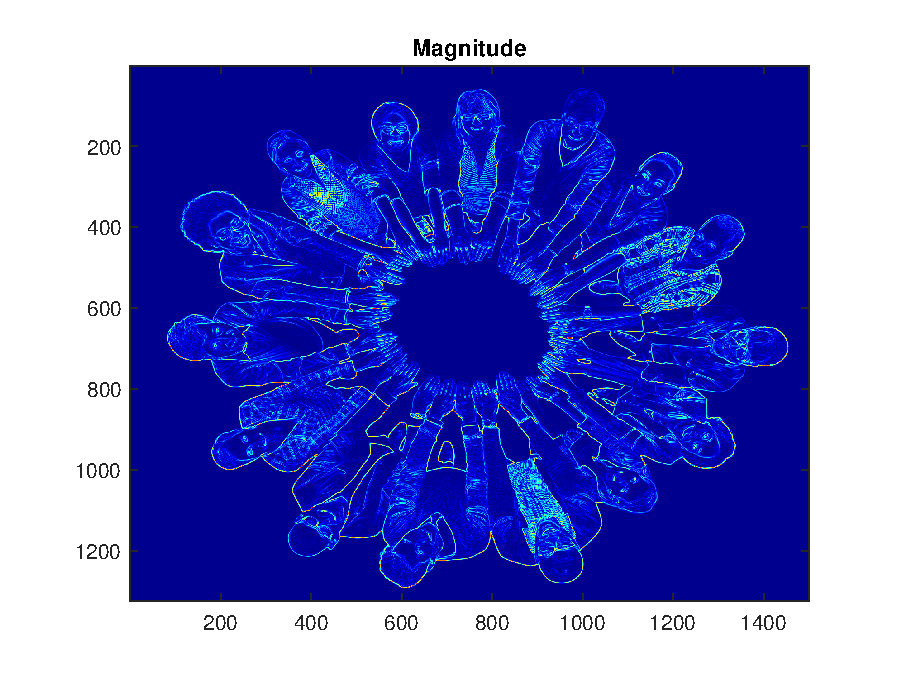
\includegraphics[width=\textwidth]{res/mag.eps}
			\caption{\tl{Magnitude of training image}}
		\end{subfigure}%
		\begin{subfigure}[b]{0.5\textwidth}
			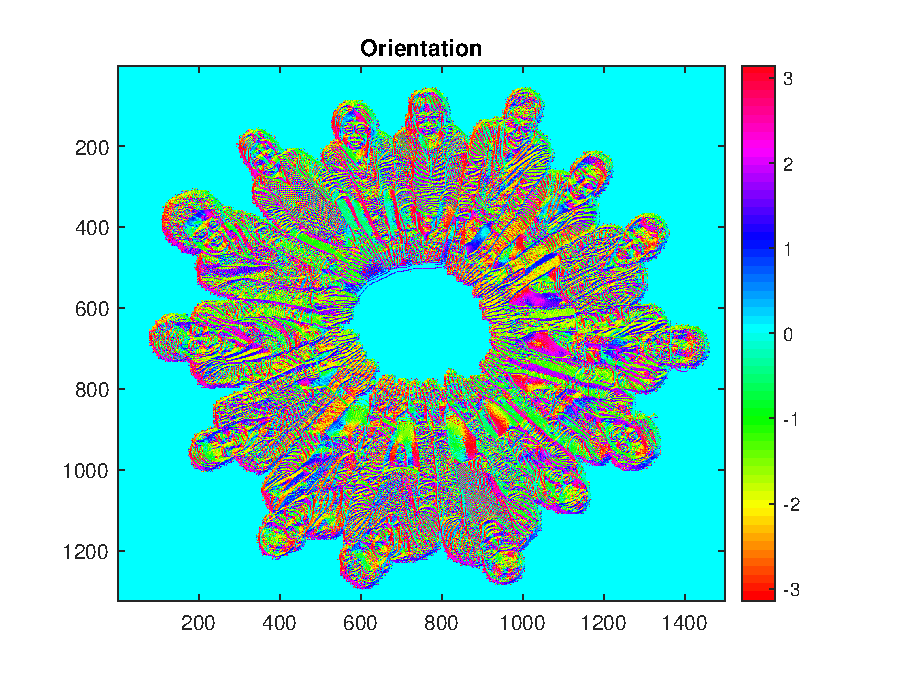
\includegraphics[width=\textwidth]{res/ori.eps}
			\caption{\tl{Orientation of training image}}
		\end{subfigure}%
		
		\begin{subfigure}[b]{0.5\textwidth}
			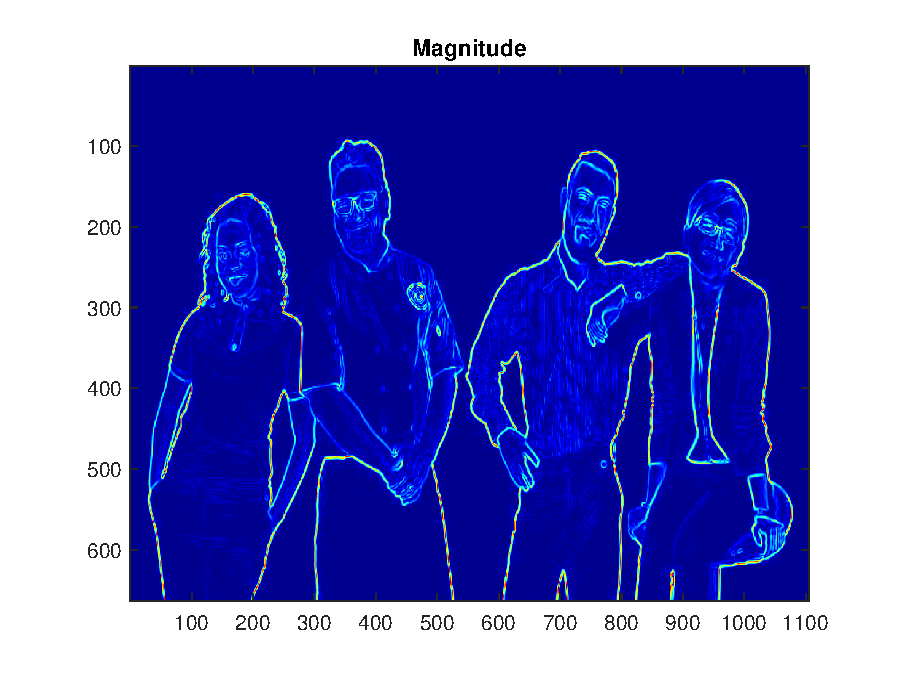
\includegraphics[width=\textwidth]{res/mag_test.eps}
			\caption{\tl{Magnitude of test image}}
		\end{subfigure}%
		\begin{subfigure}[b]{0.5\textwidth}
			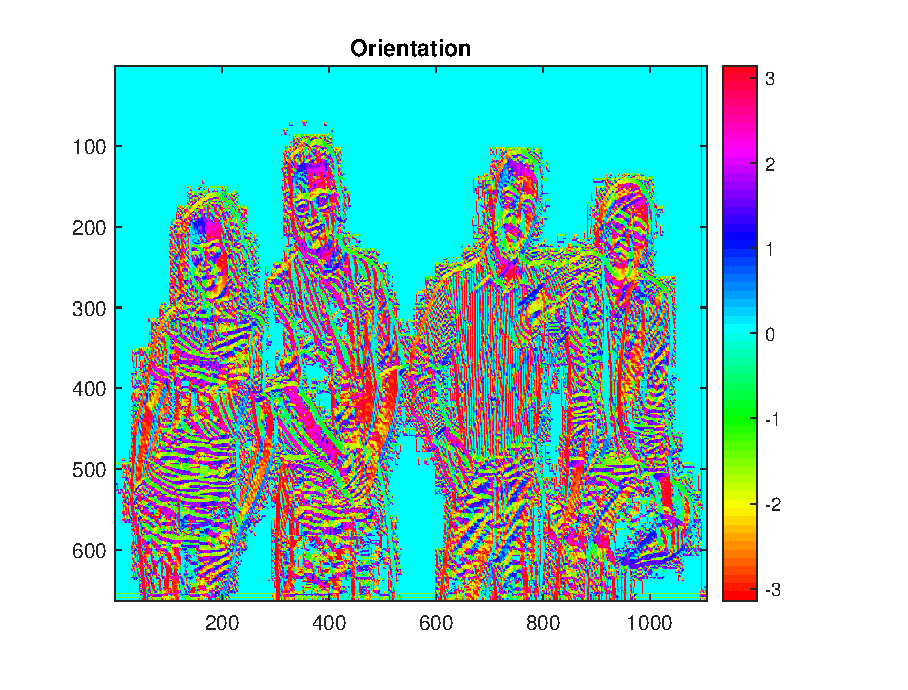
\includegraphics[width=\textwidth]{res/ori_test.eps}
			\caption{\tl{Orientation of test image}}
		\end{subfigure}%
		
		\begin{subfigure}[b]{0.5\textwidth}
			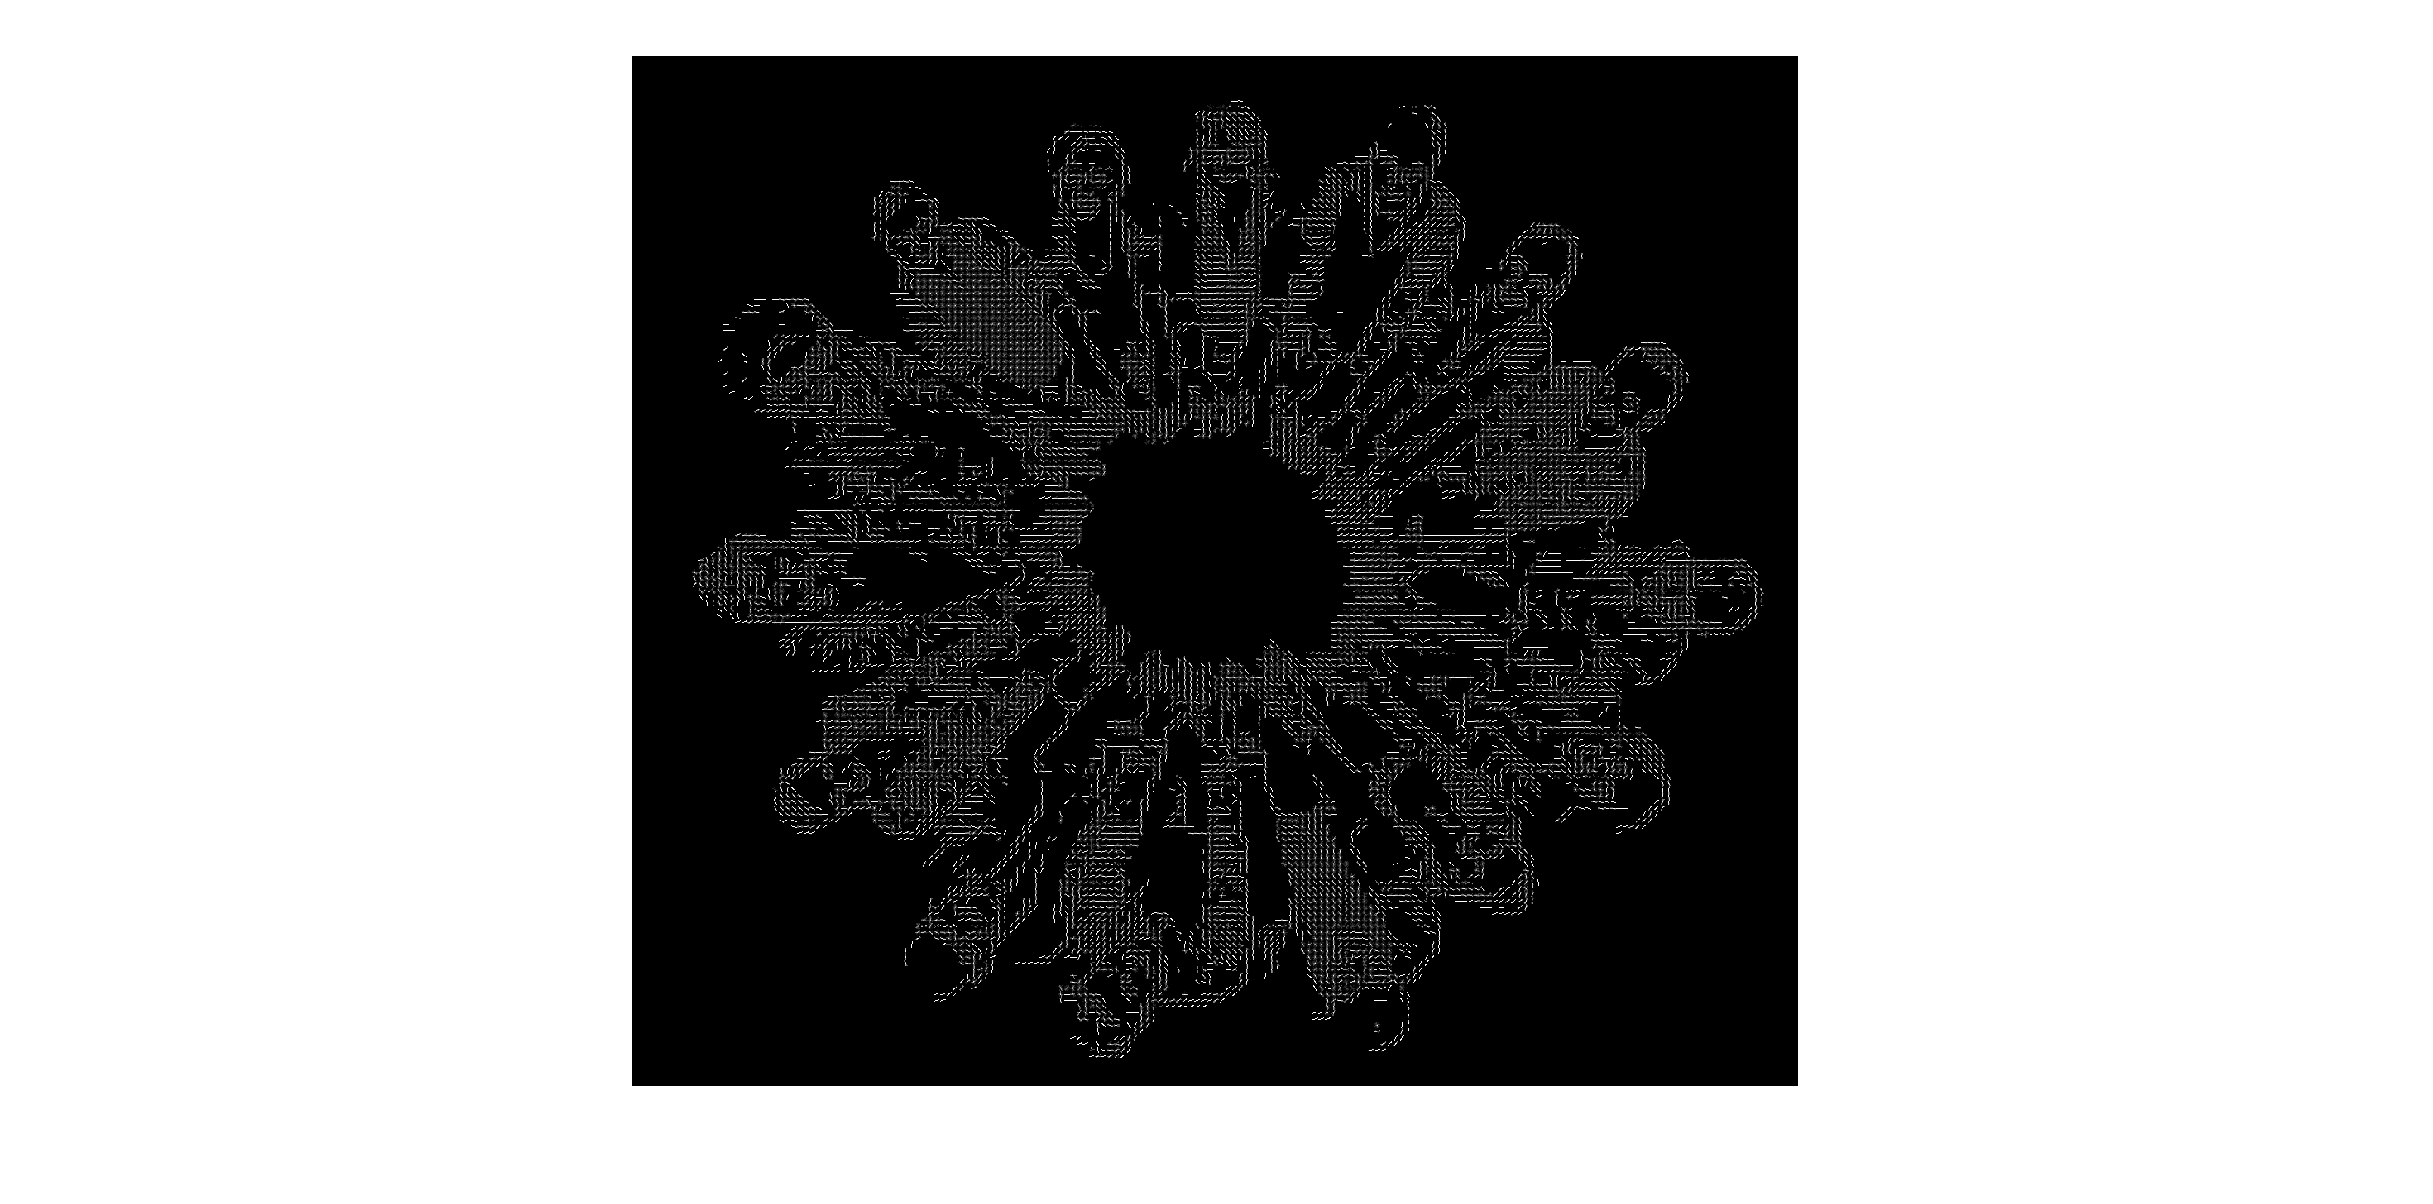
\includegraphics[width=\textwidth]{res/hogdraw_train.eps}
			\caption{\tl{Hog\_draw of training image}}		
		\end{subfigure}%
		\begin{subfigure}[b]{0.5\textwidth}
			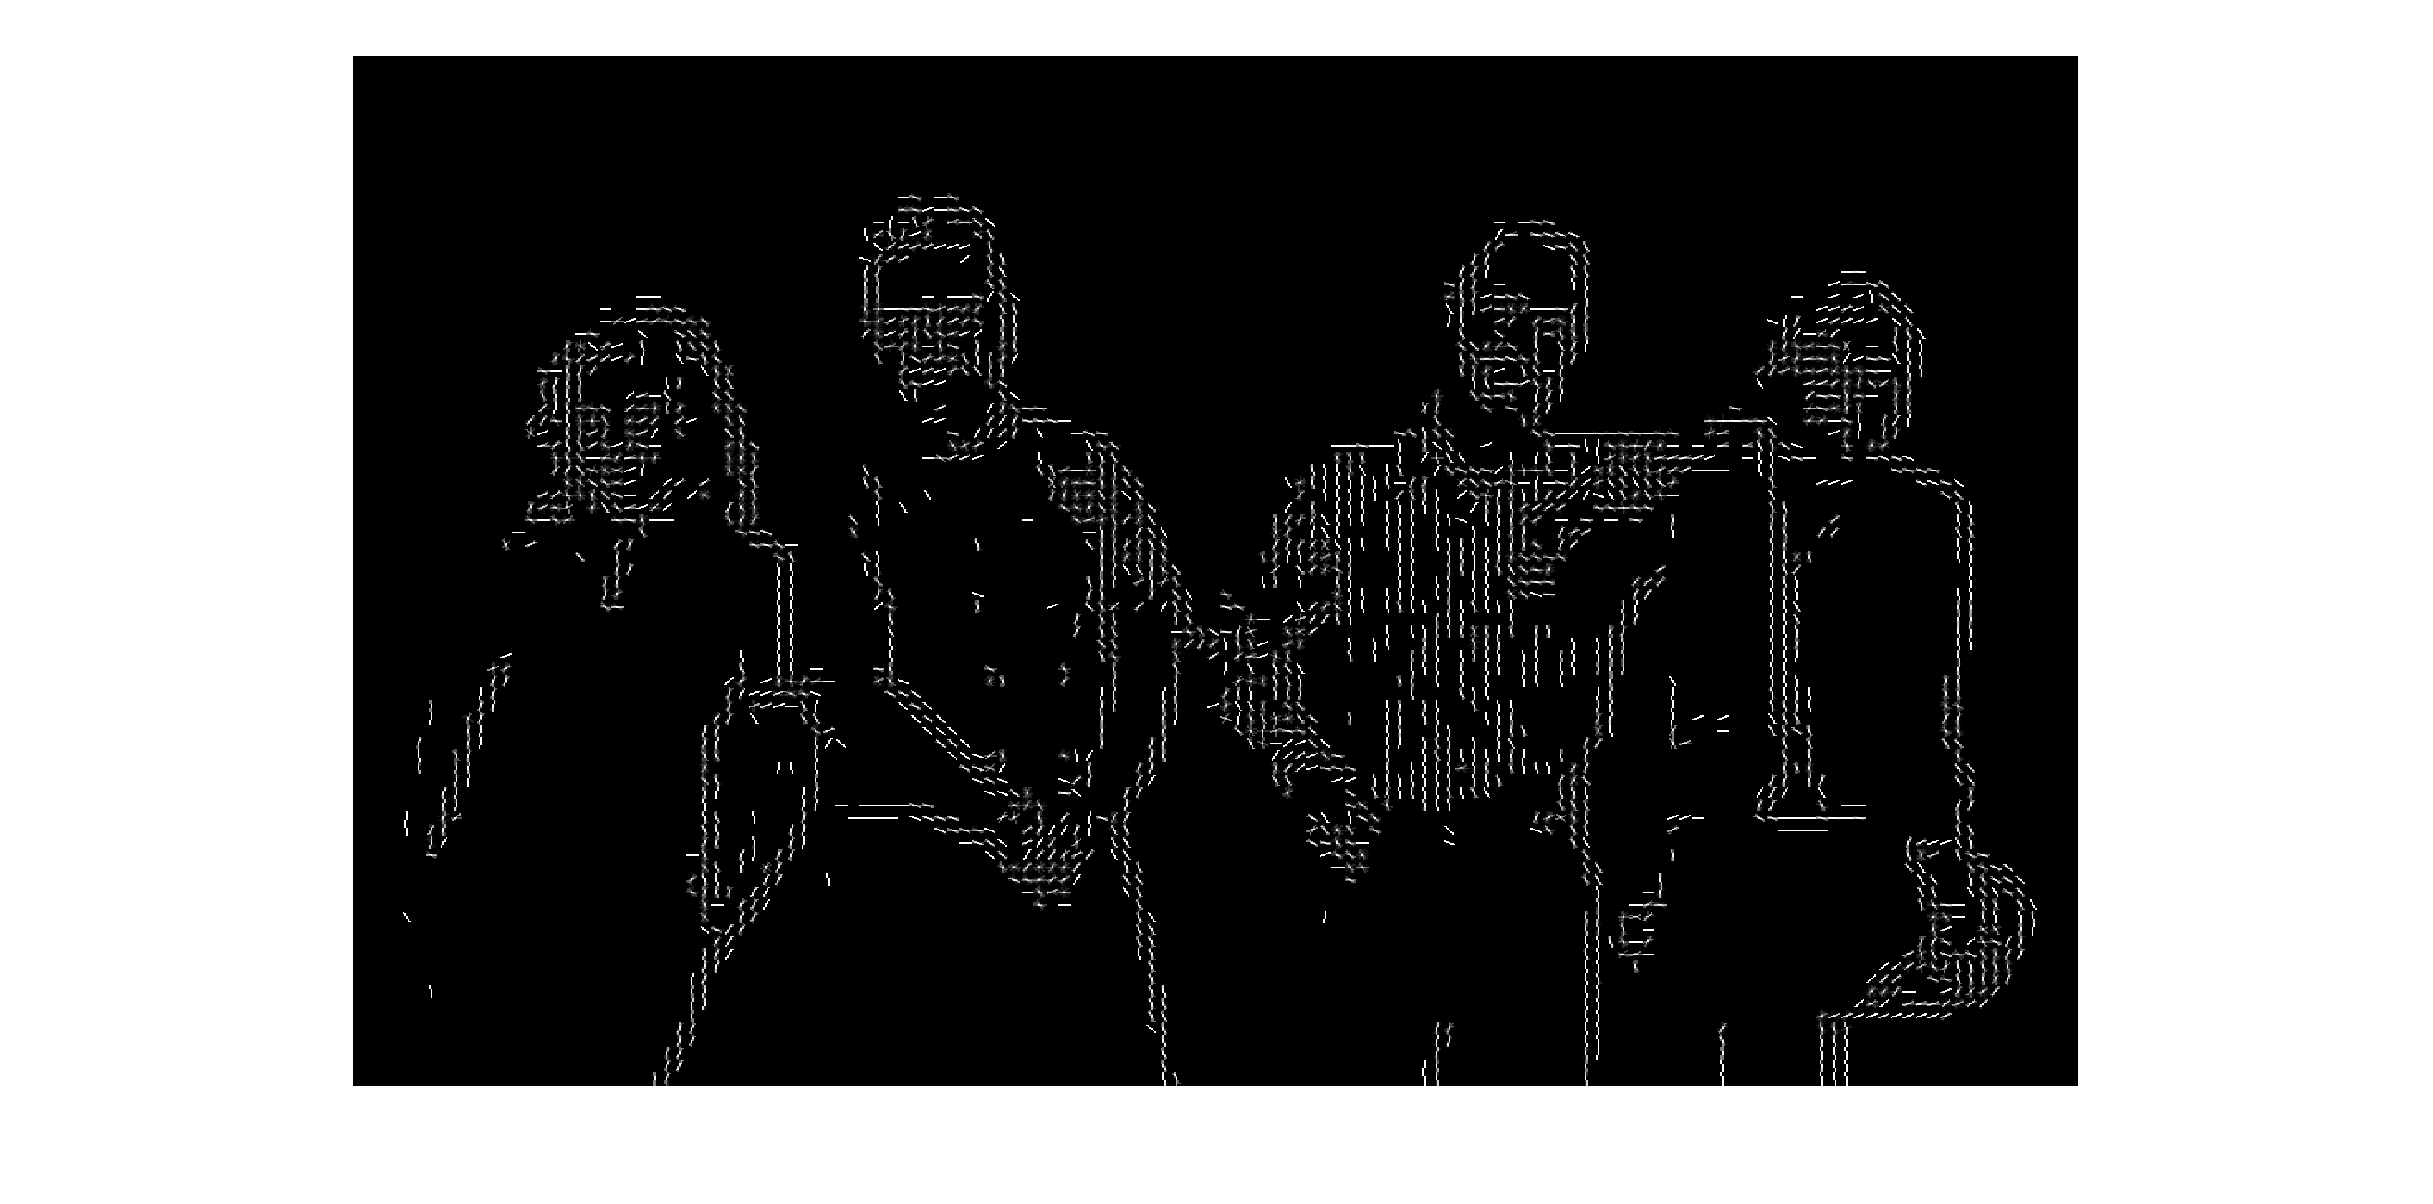
\includegraphics[width=\textwidth]{res/hogdraw_test.eps}
			\caption{\tl{Hog\_draw of test image}}	
		\end{subfigure}%	
		\caption{\tl{Algorithm's steps and results}}
		\label{fig:2}
	\end{figure}

	\begin{figure}[H]
		\centering
		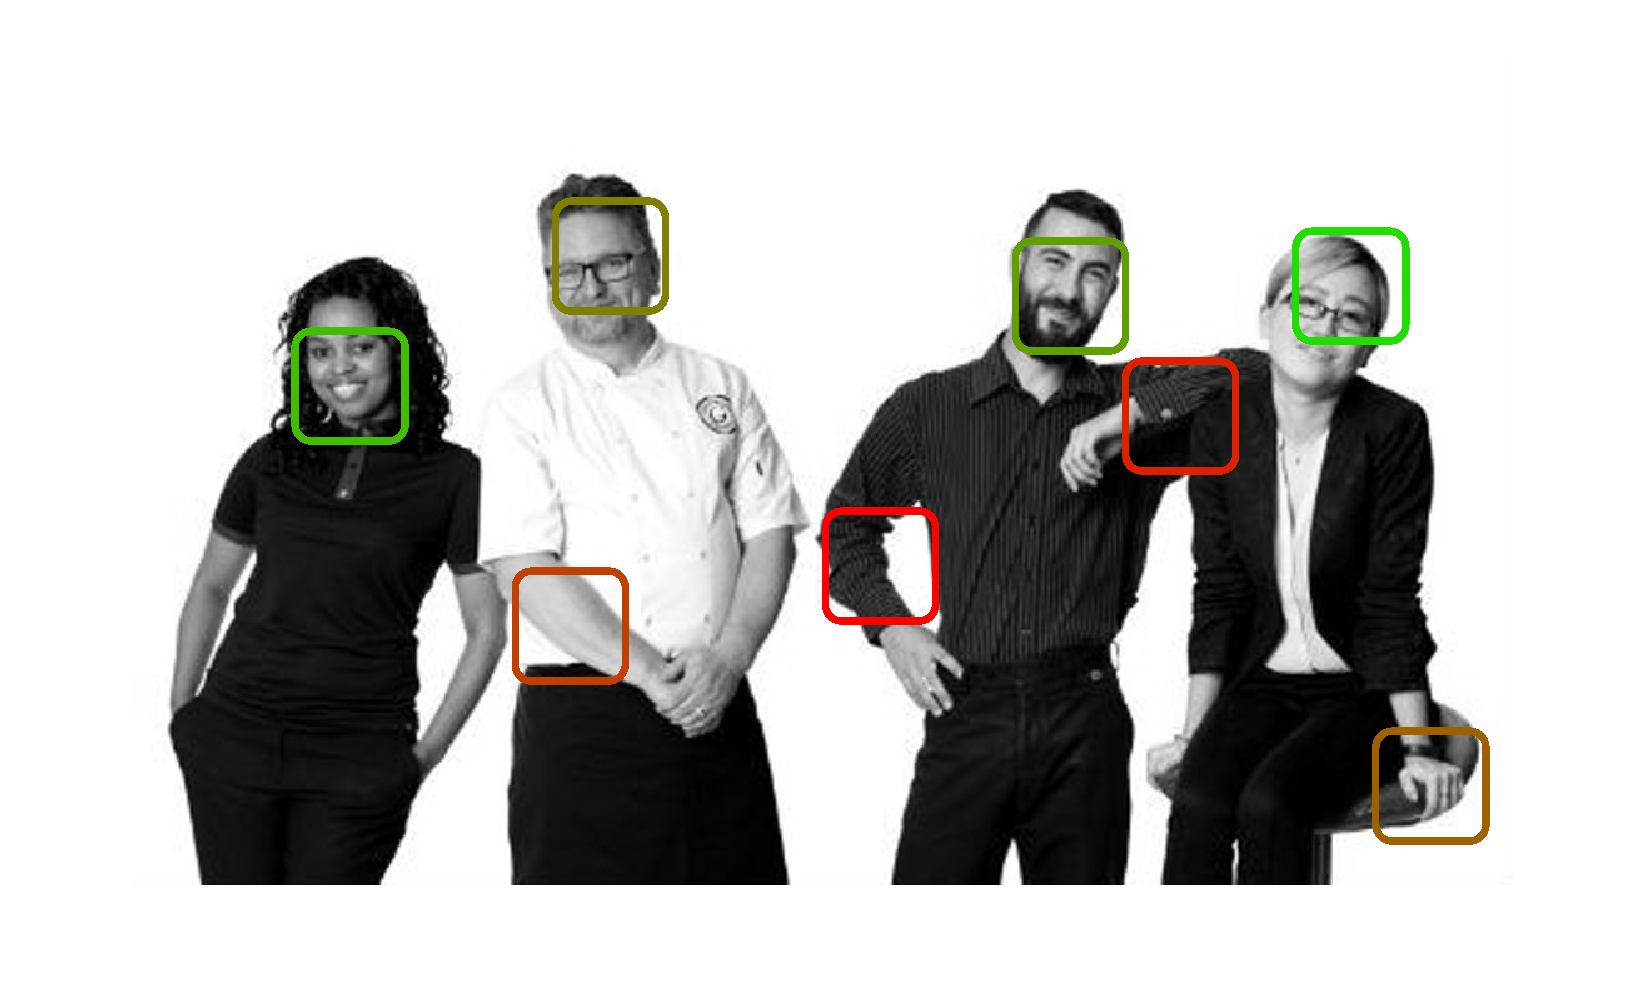
\includegraphics[scale=0.5]{res/result.eps}
		\caption{\tl{Detection with template 11x11}}
		\label{fig:3}
	\end{figure}

	\begin{figure}[H]
		\centering
		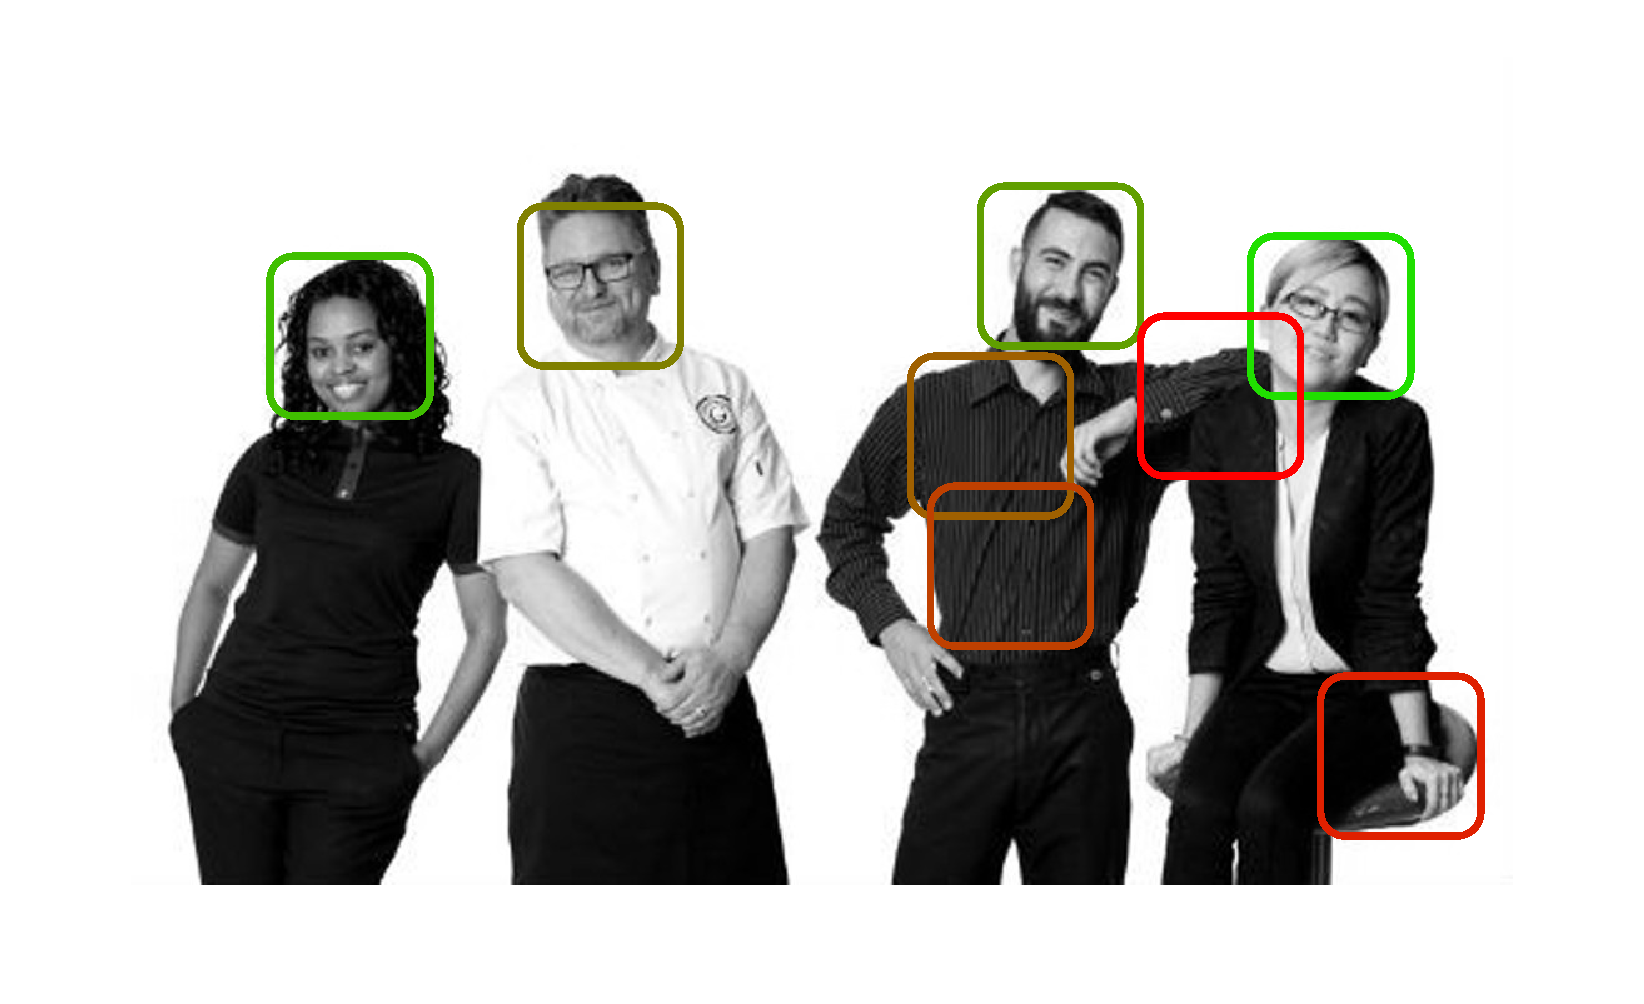
\includegraphics[scale=0.5]{res/template_size_16.eps}
		\caption{\tl{Detection with template 16x16}}
		\label{fig:4}
	\end{figure}
	
	\begin{figure}[H]
		\centering
		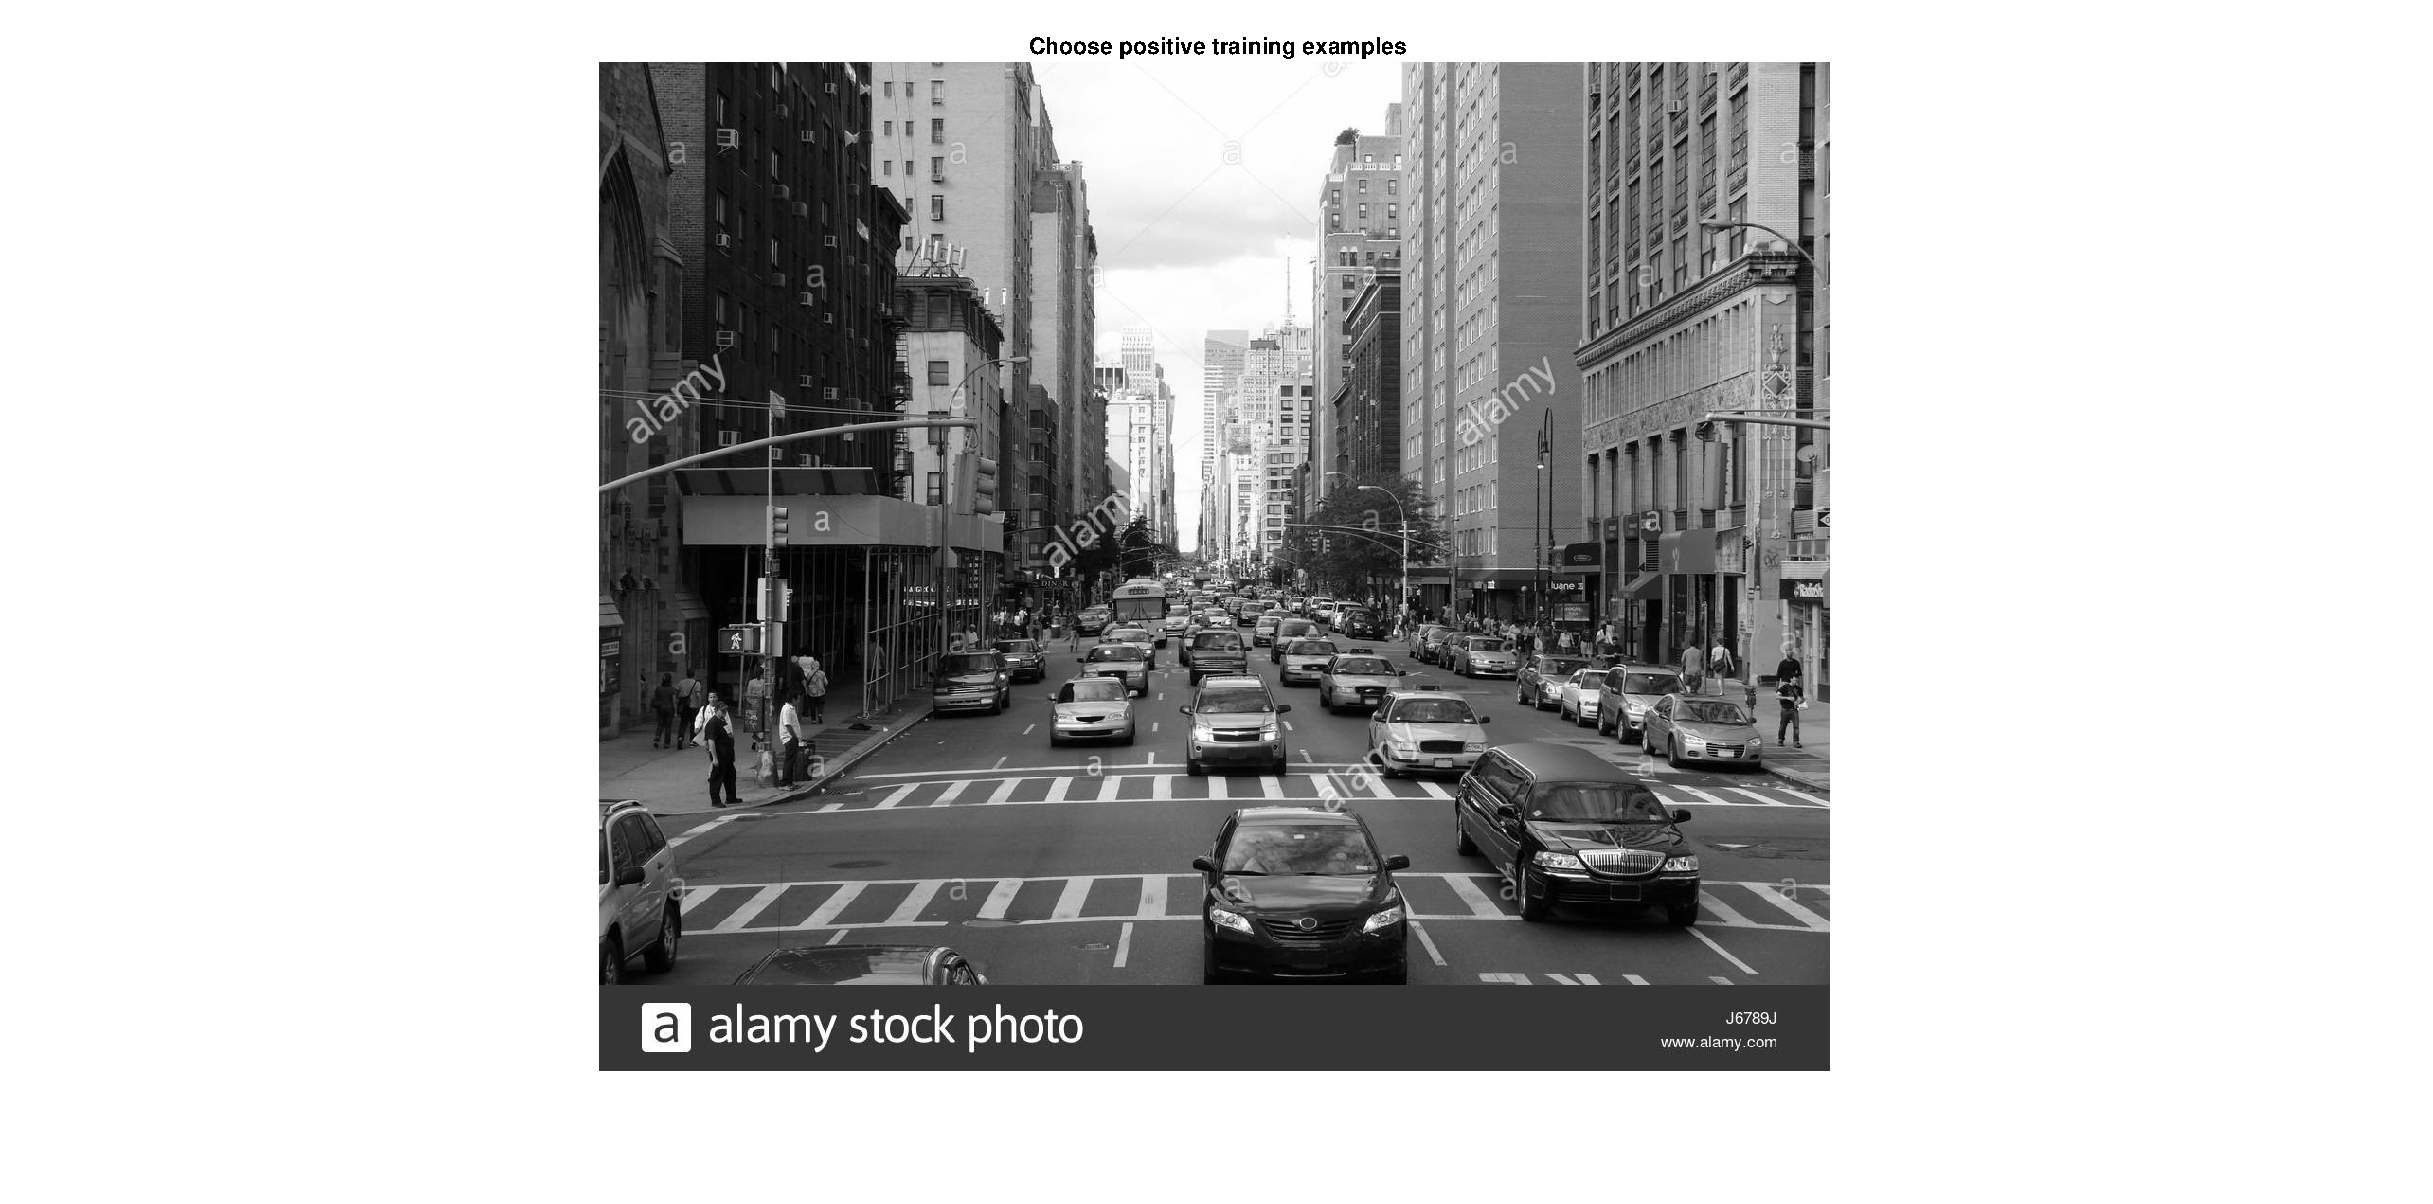
\includegraphics[scale=0.4]{res/car_15_11_input.eps}
		\caption{\tl{Input image}}
		\label{fig:5}
	\end{figure}%

	\begin{figure}[H]
		\centering
		\begin{subfigure}[b]{0.5\textwidth}
			\centering
			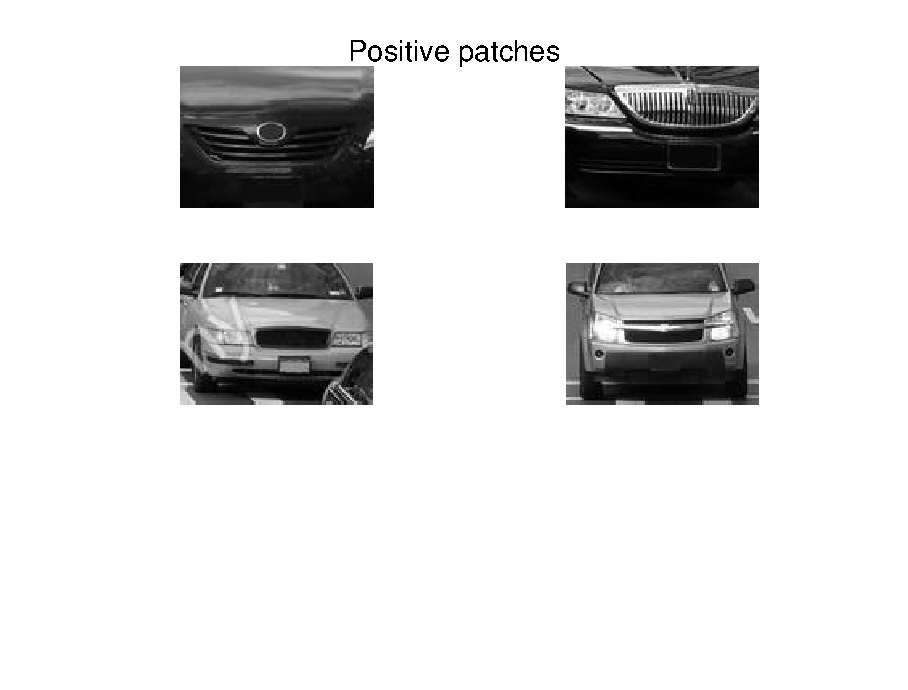
\includegraphics[width=\textwidth]{res/car_15_11_pos.eps}	
			\caption{Αυτοκίνητα προς εντοπισμό.}
		\end{subfigure}%
		\begin{subfigure}[b]{0.5\textwidth}
			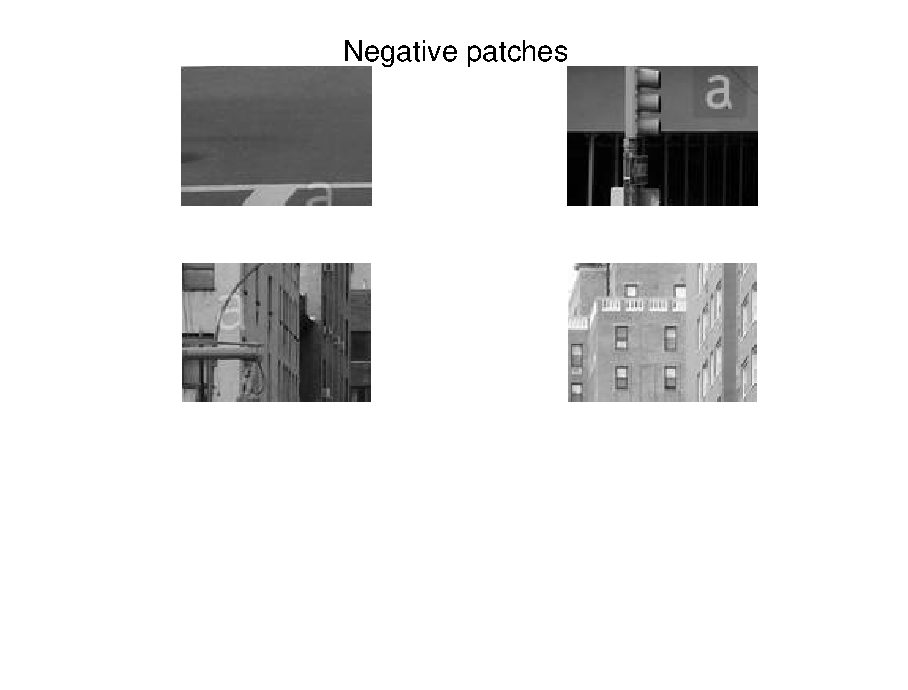
\includegraphics[width=\textwidth]{res/car_15_11_neg.eps}
			\caption{Μη επιθυμητά αντικείμενα.}
		\end{subfigure}%
		\caption{\tl{Positive and Negative patches for image \ref{fig:5}}}
		\label{fig:6}
	\end{figure}

	\begin{figure}[H]
		\centering
		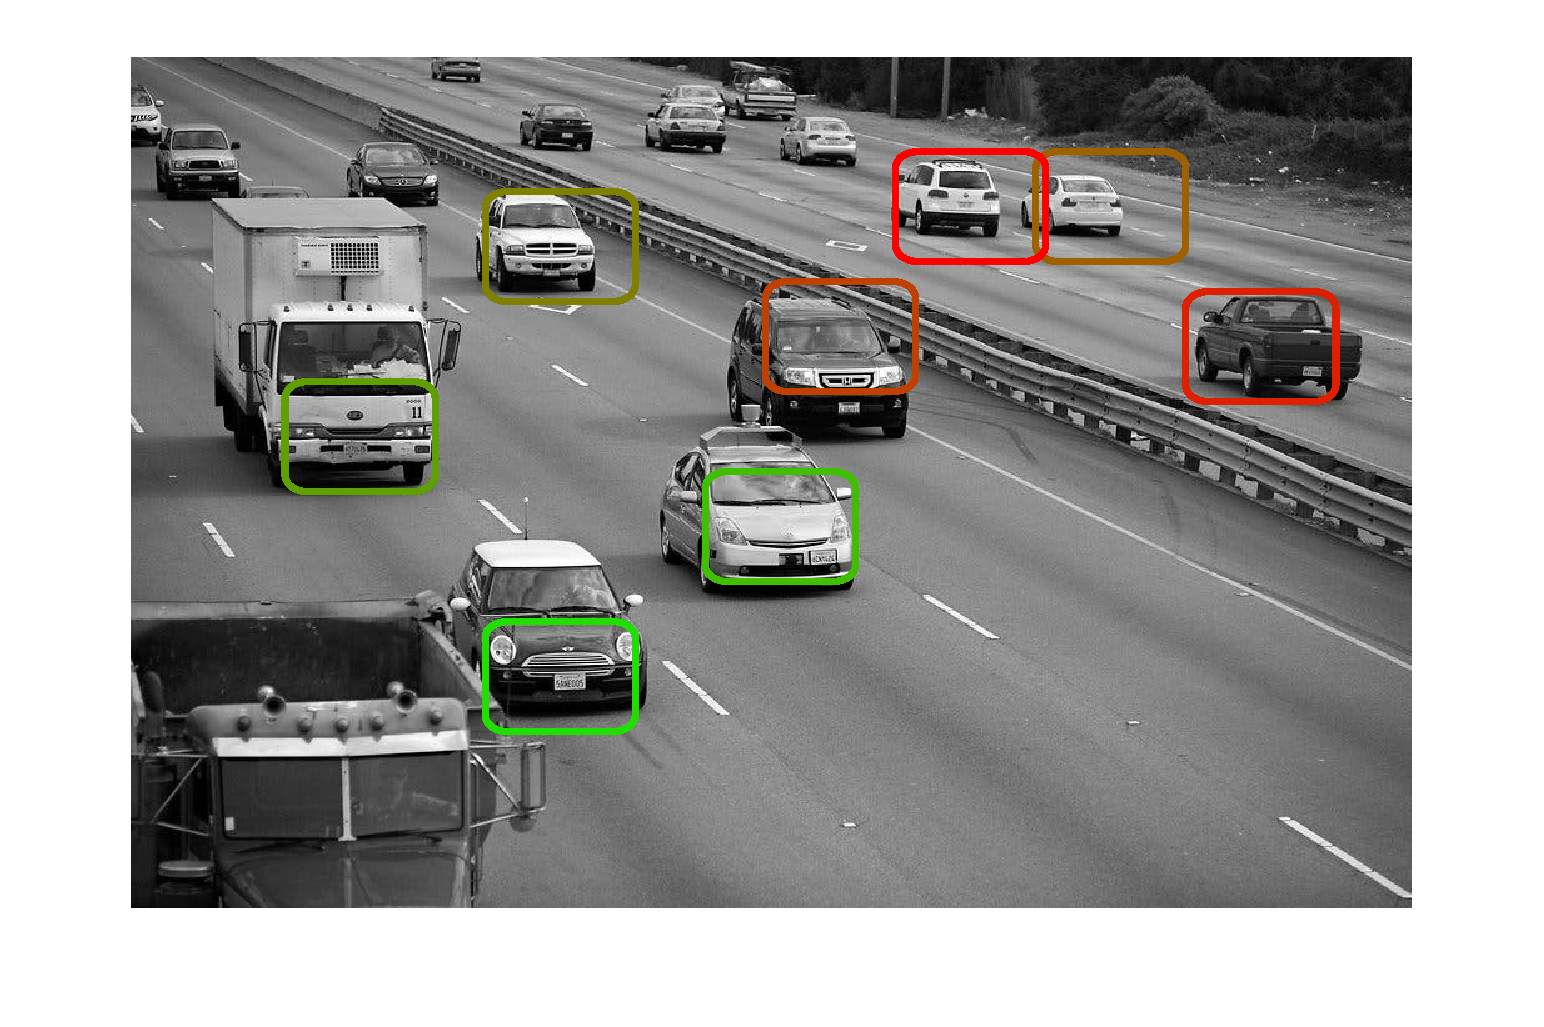
\includegraphics[scale=0.5]{res/car_15_11.eps}		
		\caption{\tl{Detection with template 15x11}}
		\label{fig:7}
	\end{figure}

	\ \\\\
	\noindent
	Aρχικά, με βάση τα \tl{positive patches} τα οποία φαίνονται στο σχήμα \ref{fig:2} \subref{fig:i}, γίνεται η αναγνώριση κάποιων άλλων 
	προσώπων στην \tl{test image} τα οποία είναι διαφορετικά από αυτά που απεικονίζονται ως \tl{positive patches}. Oι περιοχές-\tl{windows} οι οποίες έχουν το μεγαλύτερο \tl{score} (αυτές με πράσινο χρώμα) είναι 
	σε πρόσωπα που έχουν χαρακτηριστικά τα οποιία πρώτον ειναι κοινά με τα \tl{positive patches} και δευτερον δεν ανήκουν στο σύνολο των χαρακτηριστικών που δημιουργούν τα \tl{negative patches}. Παράλληλα, βλέπουμε ότι υπάρχουν και κάποια \tl{windows} που δεν βρίσκονται σε πρόσωπα και έχουν χαμηλότερο \tl{score}.  
	\\\\ 
	\noindent 
	Κατόπιν, παρατηρείται πως ακόμη και τα πιο κοντινά \tl{windows} απέχουν σημαντικά μεταξύ τους. Αυτό οφείλεται στην συνθήκη του \tl{overlap}	που κληθήκαμε να υλοποιήσουμε και αναλύθηκε στην προηγούμενη ενότητα.
	\\\\
	\noindent
	Επιπλέον, στην εικόνα \ref{fig:3} στην οποία το \tl{template} είναι 11\tl{x}11, παρατηρείται πως τα \tl{windows} o εντοπισμός των προσώπων γίνεται με μεγαλύτερη ακρίβεια σε σχέση με τα αντίστοιχα \tl{windows} για \tl{template} 16\tl{x}16 (όπως φαίνεται στην εικόνα \ref{fig:4}). Δηλαδή, αυτό που παρατηρούμε είναι ότι όσο μεγαλώνει το \tl{template size (width-heigth)} τα \tl{windows} συμπεριλαμβάνουν εκτός από τη σημαντική πληροφορία των προσώπων και πληροφορία από το λευκό \tl{background} της εικόνας.
	\\\\
	\noindent
	Τέλος, όπως φαίνεται και από την εικόνα \ref{fig:7}, έχοντας ως μεταβλητές τα \tl{width}, \tl{height} του \tl{template} έχουμε τη δηνατότητα να εντοπίσουμε αντικείμενα τα οποία έχουν σχήμα ορθοφωνίου παραλληλογράμμου. Με βάση την εικόνα \ref{fig:7} βλέπουμε ότι έχουμε έναν αρκετά ικανοποιητικό εντοπισμό των αυτοκινήτων.
\end{document} 